\section{Seguimiento y resolución de incidencias}

Una vez asignadas las incidencias, se inició el proceso de revisión y solución de los problemas reportados.

Para el Issue \#7, correspondiente al problema de inicio de sesión, primero se consultó la información de la incidencia y posteriormente se agregó un comentario indicando el inicio de la revisión.

\begin{lstlisting}
gh issue view 7 --repo martinezmoralesdiego2020-droid/repositorio

gh issue comment 7 \
--repo martinezmoralesdiego2020-droid/repositorio \
--body "Se inicia la revision del problema de inicio de sesion."
\end{lstlisting}

\begin{figure}[H]
\centering
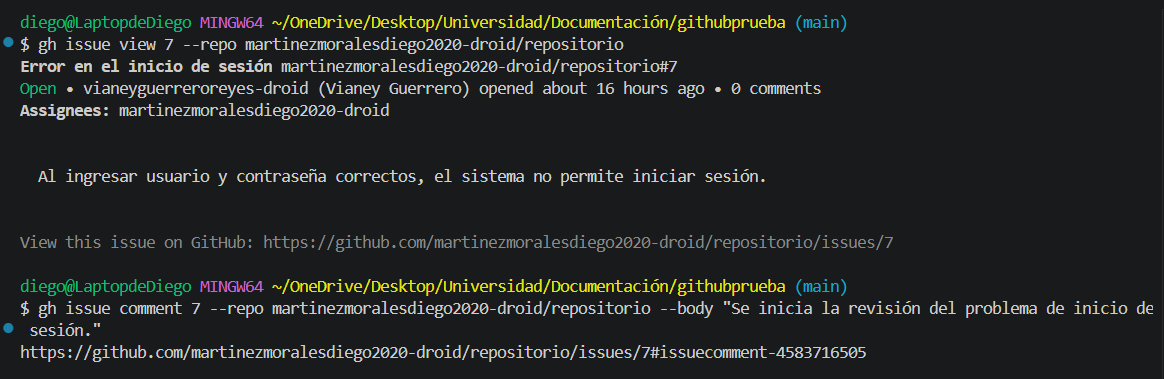
\includegraphics[width=0.9\textwidth]{M11.png}
\caption{Consulta y comentario inicial del Issue \#7.}
\end{figure}

Posteriormente se cambió a la rama correspondiente para realizar la corrección, se registraron los cambios mediante un commit y se enviaron al repositorio remoto.

\begin{lstlisting}
git switch fix-issue-7
git add .
git commit -m "Fix #7: corregido problema de inicio de sesion"
git push origin fix-issue-7
\end{lstlisting}

Finalmente, una vez concluida la corrección, la incidencia fue cerrada agregando un comentario que documenta su solución.

\begin{lstlisting}
gh issue close 7 \
--repo martinezmoralesdiego2020-droid/repositorio \
--comment "Problema de inicio de sesion revisado y corregido."
\end{lstlisting}

\begin{figure}[H]
\centering
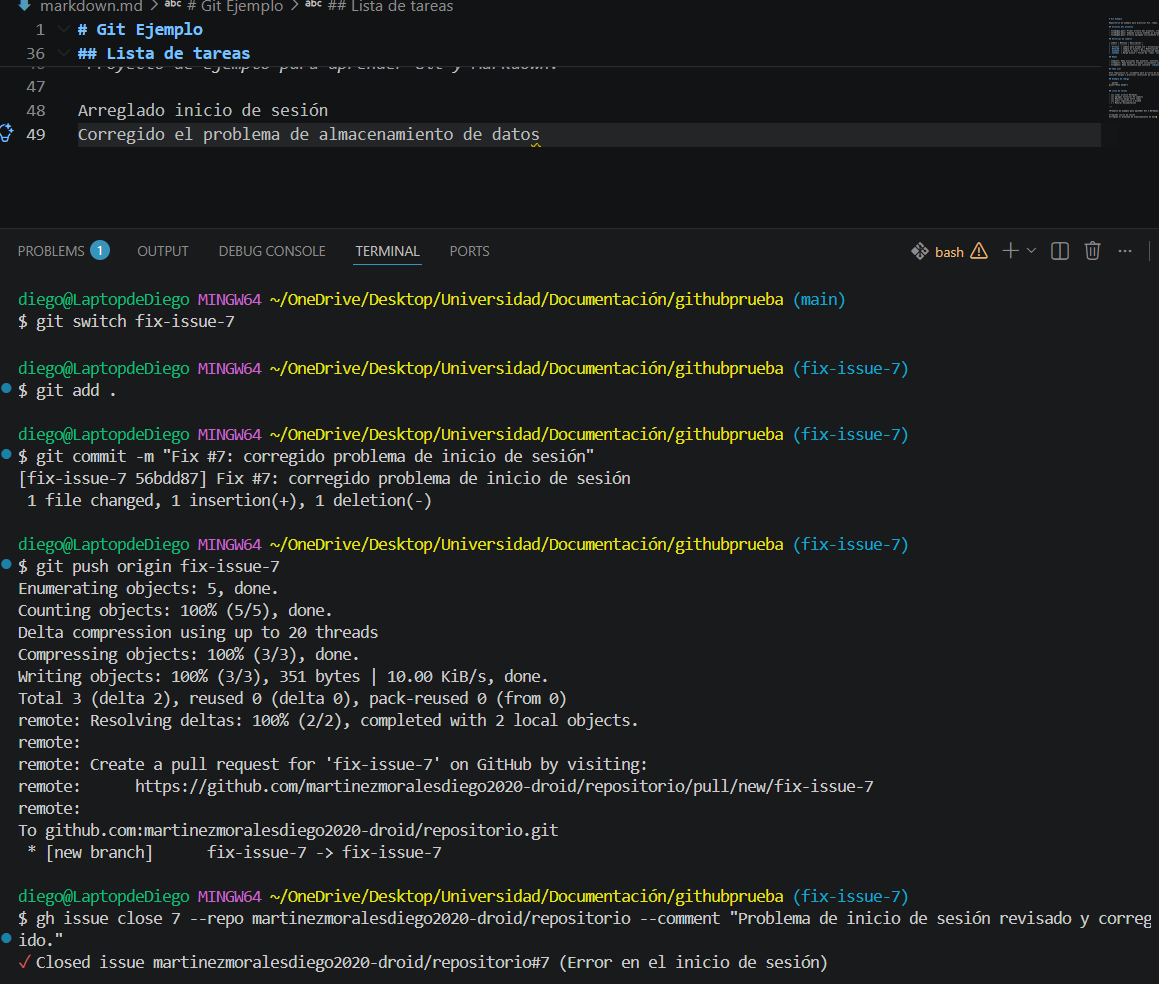
\includegraphics[width=0.9\textwidth]{M12.png}
\caption{Proceso de corrección y cierre del Issue \#7.}
\end{figure}

De forma similar, se realizó el seguimiento del Issue \#8 relacionado con el almacenamiento de datos. Inicialmente se consultó la incidencia y se registró un comentario indicando el comienzo de la revisión.

\begin{lstlisting}
gh issue view 8 --repo martinezmoralesdiego2020-droid/repositorio

gh issue comment 8 \
--repo martinezmoralesdiego2020-droid/repositorio \
--body "Se inicia la revision del problema de almacenamiento de datos."
\end{lstlisting}

\begin{figure}[H]
\centering
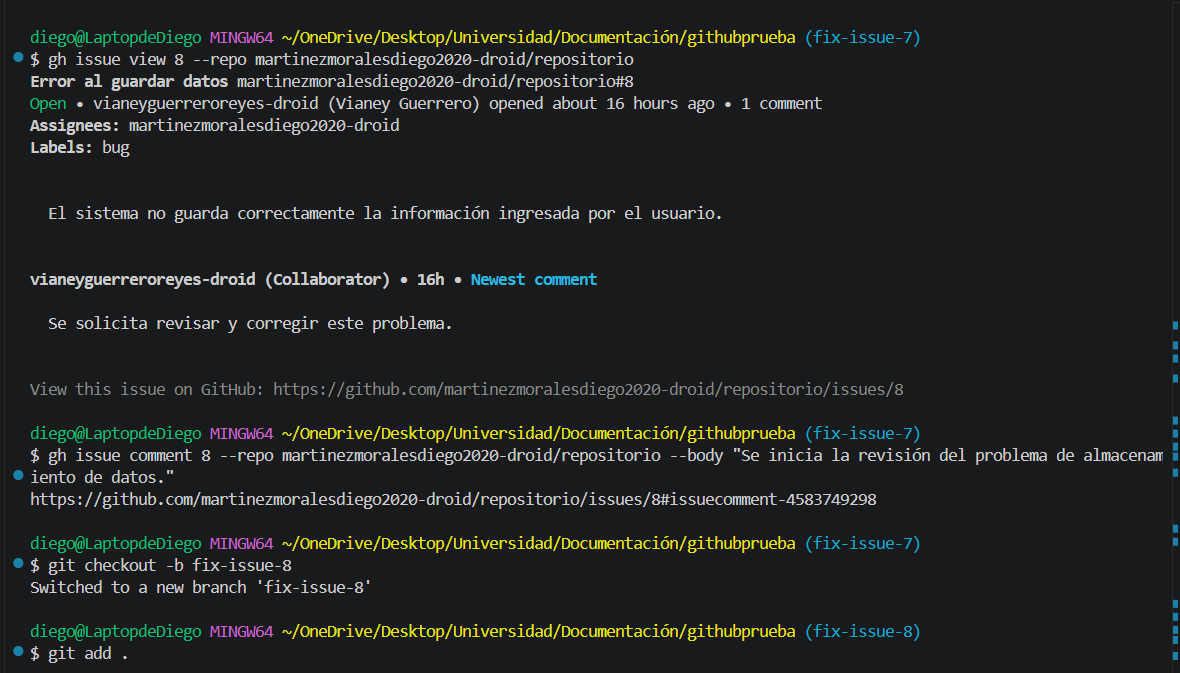
\includegraphics[width=0.9\textwidth]{M13.png}
\caption{Consulta y comentario inicial del Issue \#8.}
\end{figure}

Posteriormente se creó una rama específica para la corrección, se realizaron los cambios correspondientes y se enviaron al repositorio remoto.

\begin{lstlisting}
git checkout -b fix-issue-8
git add .
git commit -m "Fix #8: corregido problema de almacenamiento de datos"
git push origin fix-issue-8
\end{lstlisting}

Una vez finalizada la corrección, la incidencia fue cerrada mediante GitHub CLI dejando evidencia de la solución aplicada.

\begin{lstlisting}
gh issue close 8 \
--repo martinezmoralesdiego2020-droid/repositorio \
--comment "Problema de almacenamiento revisado y corregido."
\end{lstlisting}

\begin{figure}[H]
\centering
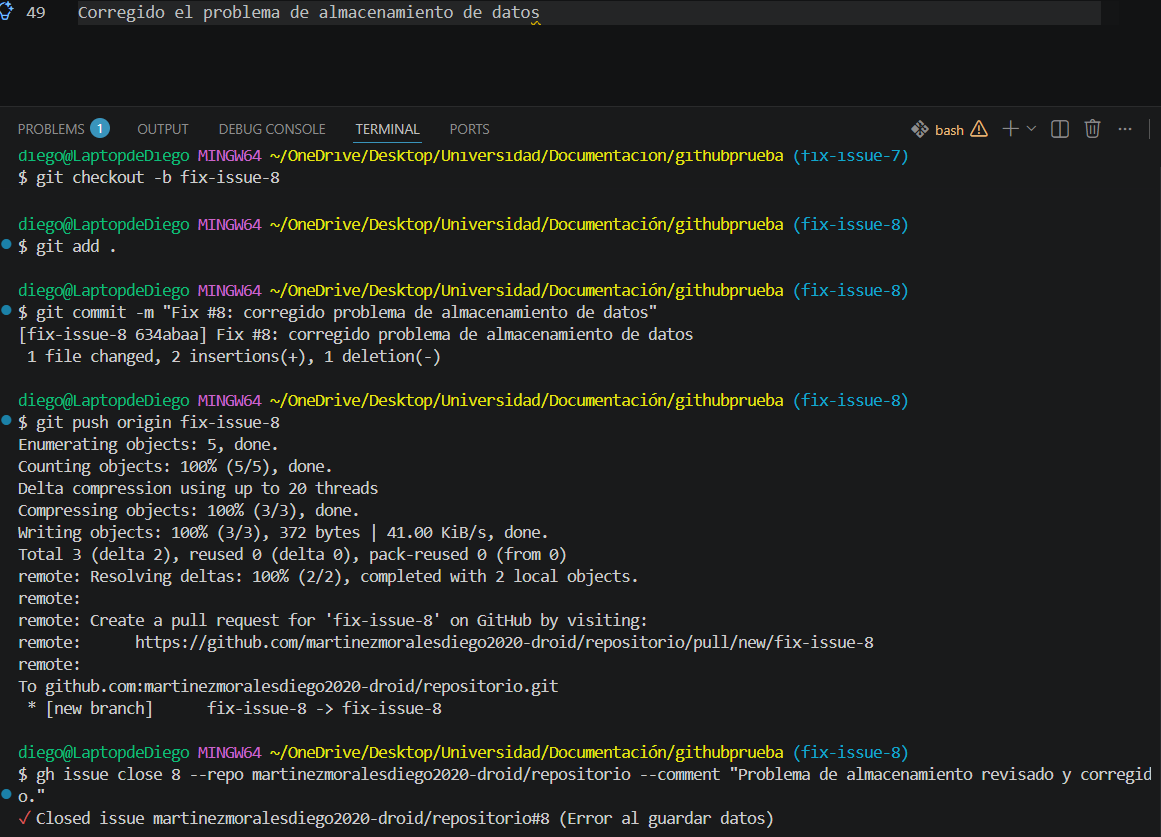
\includegraphics[width=0.9\textwidth]{M14.png}
\caption{Proceso de corrección y cierre del Issue \#8.}
\end{figure}

Finalmente se verificó desde la interfaz web de GitHub que ambas incidencias aparecieran como cerradas, confirmando que el flujo de trabajo había sido completado correctamente.

\begin{figure}[H]
\centering
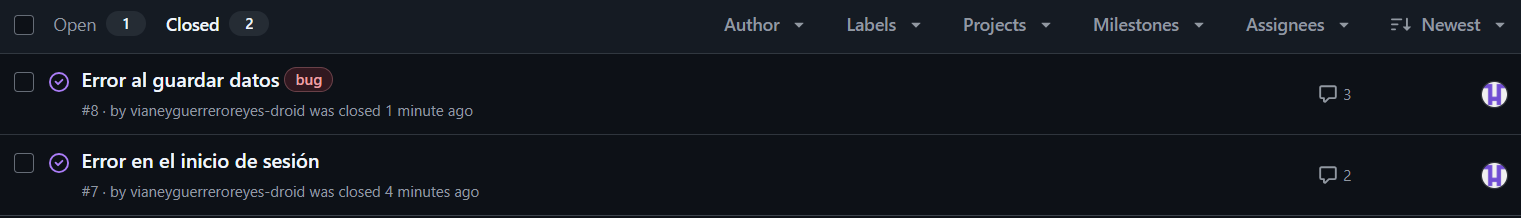
\includegraphics[width=0.9\textwidth]{M15.png}
\caption{Listado de incidencias cerradas en GitHub.}
\end{figure}

También se revisó el historial de cada incidencia para comprobar que los comentarios, asignaciones y cierre hubieran quedado registrados correctamente.

\begin{figure}[H]
\centering
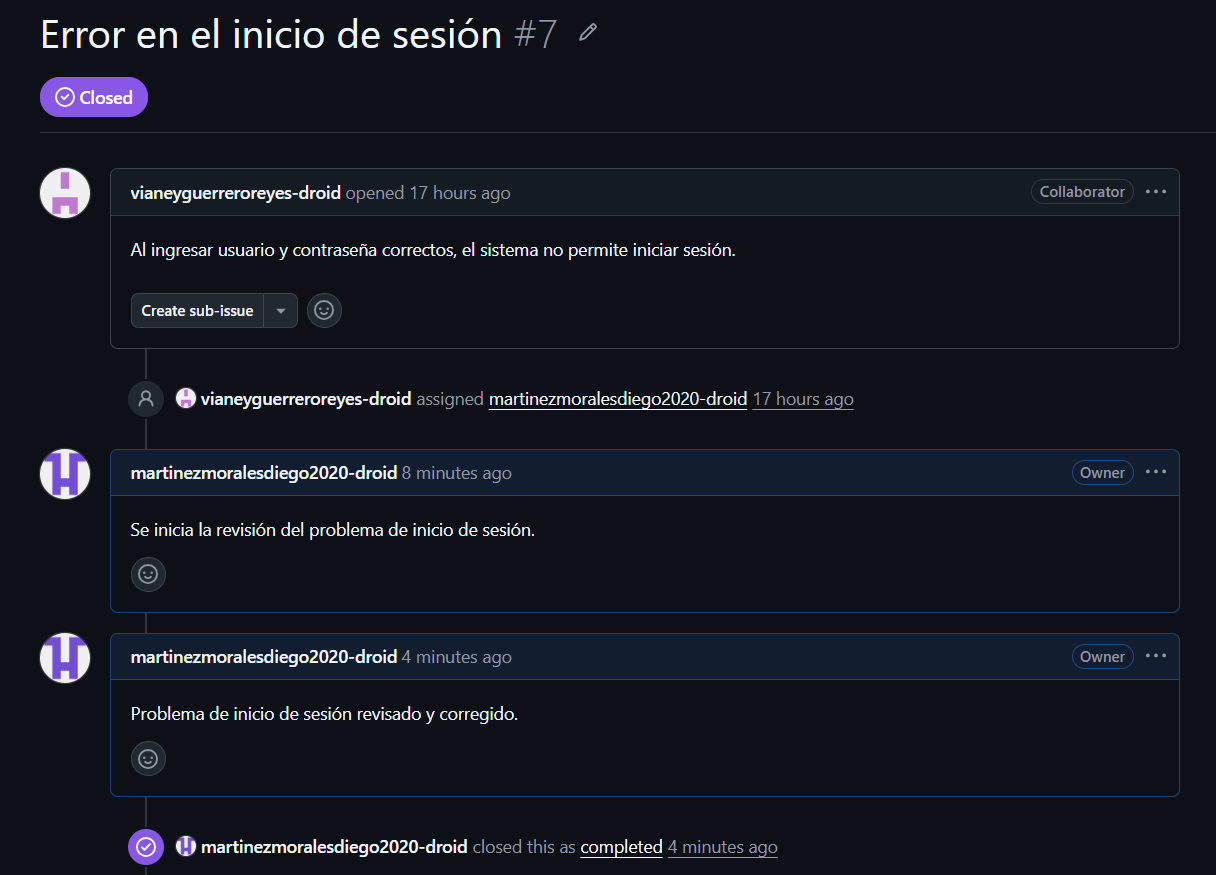
\includegraphics[width=0.9\textwidth]{M16.png}
\caption{Historial completo del Issue \#7 después de su resolución.}
\end{figure}

\begin{figure}[H]
\centering
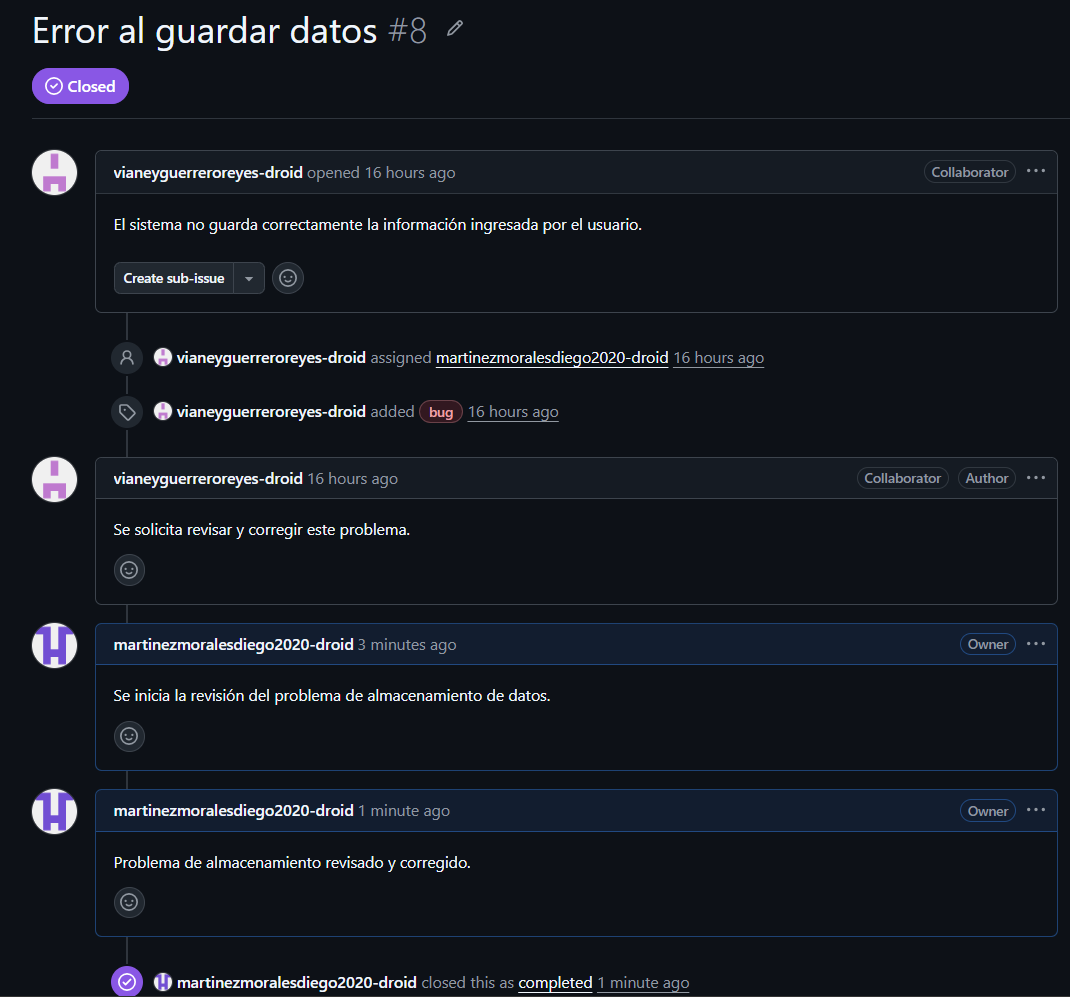
\includegraphics[width=0.9\textwidth]{M17.png}
\caption{Historial completo del Issue \#8 después de su resolución.}
\end{figure}